\documentclass[12pt,a4paper]{report}
\usepackage[margin=1in]{geometry}
\usepackage[T1]{fontenc}
\usepackage{lmodern}
\usepackage{microtype}
\usepackage{setspace}
\usepackage{xcolor}
\usepackage{graphicx}
\usepackage{booktabs}
\usepackage{tabularx}
\usepackage{array}
\usepackage{enumitem}
\usepackage{amsmath}
\usepackage{hyperref}
\usepackage{fancyhdr}
\usepackage{titlesec}
\usepackage{float}
\usepackage{caption}
\usepackage{parskip}

\definecolor{aublue}{HTML}{17324D}
\definecolor{auteal}{HTML}{167D8D}
\hypersetup{colorlinks=true,linkcolor=aublue,urlcolor=auteal,citecolor=aublue,pdftitle={Hostel Mess Menu Optimizer}}
\setstretch{1.16}
\setlist[itemize]{leftmargin=1.45em,itemsep=0.25em,topsep=0.35em}
\setlist[enumerate]{leftmargin=1.6em,itemsep=0.25em,topsep=0.35em}
\titleformat{\chapter}{\normalfont\huge\bfseries\color{aublue}}{\thechapter.}{0.55em}{}
\titleformat{\section}{\normalfont\Large\bfseries\color{aublue}}{\thesection}{0.55em}{}
\pagestyle{fancy}
\fancyhf{}
\lhead{Hostel Mess Menu Optimizer}
\rhead{Soft Computing Project}
\cfoot{\thepage}
\renewcommand{\headrulewidth}{0.3pt}
\newcolumntype{Y}{>{\raggedright\arraybackslash}X}

\begin{document}
\begin{titlepage}
\centering
\vspace*{1.1cm}
{\Large \textbf{ADANI UNIVERSITY} \par}
\vspace{0.25cm}
{\large Department of Computer Science and Engineering \par}
\vfill
{\color{auteal}\rule{0.76\textwidth}{1.2pt}\par}
\vspace{0.6cm}
{\Huge\bfseries Hostel Mess Menu Optimizer\par}
\vspace{0.35cm}
{\Large A Multi-Objective Evolutionary Approach for Weekly and Monthly Meal Planning\par}
\vspace{0.6cm}
{\color{auteal}\rule{0.76\textwidth}{1.2pt}\par}
\vfill
\begin{tabular}{rl}
\textbf{Course:} & Soft Computing\\[0.3cm]
\textbf{Submitted by:} & Rishi Raval \hspace{1.2cm} (1AUA23BCS155)\\
& Drashti Sojitra \hspace{0.8cm} (1AUA24BCS921)\\[0.3cm]
\textbf{Faculty/Guide:} & \textit{[To be added]}\\[0.3cm]
\textbf{Semester:} & 7th Semester\\
\textbf{Academic Year:} & 2026--27
\end{tabular}
\vfill
{\large Submitted in partial fulfilment of the course requirements for Soft Computing\par}
\vspace*{0.7cm}
\end{titlepage}

\pagenumbering{roman}
\tableofcontents
\listoffigures
\listoftables
\clearpage
\pagenumbering{arabic}

\chapter{Abstract}
Planning a hostel mess menu is a small decision with a large daily impact. A menu must stay within budget, provide reasonable nutrition, respect meal-slot suitability, and avoid serving the same dish too often. These needs conflict: the least expensive menu is not automatically the most balanced or the most appealing. This project develops a \textit{Hostel Mess Menu Optimizer} that produces feasible weekly menus and then selects four sufficiently different weeks for a monthly plan.

The system uses NSGA-II, a multi-objective evolutionary algorithm. Rather than forcing cost, nutrition and student preference into one arbitrary score, it returns several non-dominated alternatives. Each weekly candidate has 21 selections: breakfast, lunch and dinner for seven days. The evaluator checks daily calorie bounds, daily cost cap, vegetarian policy, slot eligibility and repetition rules before a candidate can be recommended. A four-week selector then rejects duplicate or overly similar schedules.

The implementation uses a dataset of 200 vegetarian hostel meal options and a Python backend with a React-based student interface. In a ten-seed benchmark, NSGA-II found feasible candidates in every run and produced a mean of 13.2 non-dominated menus. The reported results are planning outputs, not medical advice: nutritional values are recipe estimates and current ratings are synthetic. The project demonstrates how soft computing can support a transparent, practical planning task where there is no single perfect answer.

\chapter{Introduction}
\section{Background and motivation}
A hostel menu is usually planned with a spreadsheet, familiar recipes and a manual sense of balance. That approach is understandable, but it becomes difficult when several conditions must be checked together. A dish that fits breakfast may not fit dinner; a cheap day can be nutritionally weak; and a menu that repeats familiar items may lead to dissatisfaction.

This project treats menu planning as a constrained decision problem. It is similar to choosing a route: the shortest route may not be the fastest, safest or most pleasant. In the same way, the cheapest menu may not be the best overall menu. The aim is to offer the mess manager a small set of sensible trade-offs rather than claim that one menu is universally best.

\section{Importance and overview}
The system is relevant to hostel operations because it makes the decision process repeatable and visible. A weekly plan is encoded as 21 meal choices. A rule-checking engine evaluates it, NSGA-II searches for good alternatives, and a monthly selector chooses diverse weeks. The student-facing interface displays the generated plan through a FastAPI service and React frontend.

\chapter{Problem Statement \& Objectives}
\section{Problem statement}
Given a catalogue of hostel meals, generate weekly vegetarian menus that keep daily spending within a limit, satisfy basic calorie bounds, match breakfast/lunch/dinner suitability, avoid nearby repetitions, and balance nutrition with estimated student preference. From feasible weekly menus, select four weeks that are not near copies of one another.

\section{Objectives}
\begin{itemize}
\item Represent a seven-day, three-meal-per-day menu in a form suitable for evolutionary search.
\item Evaluate cost, nutrition deviation and dissatisfaction for every candidate menu.
\item Enforce operational rules as hard constraints before recommending a menu.
\item Use NSGA-II to expose useful trade-offs instead of hiding them in a single score.
\item Compare the optimizer with random feasible and greedy-cost baselines.
\item Build a simple web interface that can request, view and export generated plans.
\item Select four weekly schedules with a configurable minimum difference between them.
\end{itemize}

\chapter{Literature Review / Existing Work}
Meal planning is commonly approached through manual planning, rule-based selection, or single-objective optimization. Manual plans use practical experience but can miss a constraint when schedules become large. Rule-based systems are transparent, yet they generally return the first acceptable answer and do not show alternatives. Linear or integer programming can be effective when all priorities can be expressed in one fixed objective, but selecting the relative importance of cost, nutrition and preference is difficult.

Evolutionary multi-objective methods are useful when objectives compete. Deb et al. introduced NSGA-II as an efficient way to retain diverse, non-dominated solutions \cite{deb2002}. In food and diet planning, optimization has also been used to manage nutritional targets and cost \cite{ferguson2004}. This project differs in its practical focus: it adds meal-slot validity, a short repetition window, a vegetarian policy, a daily cost cap, and a second layer that checks diversity across four weekly plans. It does not claim clinical diet optimization; it is a hostel planning tool using estimated meal data.

\chapter{Proposed Methodology}
\section{Overall approach}
The process begins with a cleaned meal dataset. The loader creates stable meal identifiers and eligible choices for each slot. The evaluator converts a 21-item candidate into a readable weekly schedule, calculates objectives, and records every violated rule. NSGA-II evolves candidates through slot-aware initialization, crossover and mutation. Finally, feasible non-dominated menus are passed to the monthly selector.

\begin{figure}[H]
\centering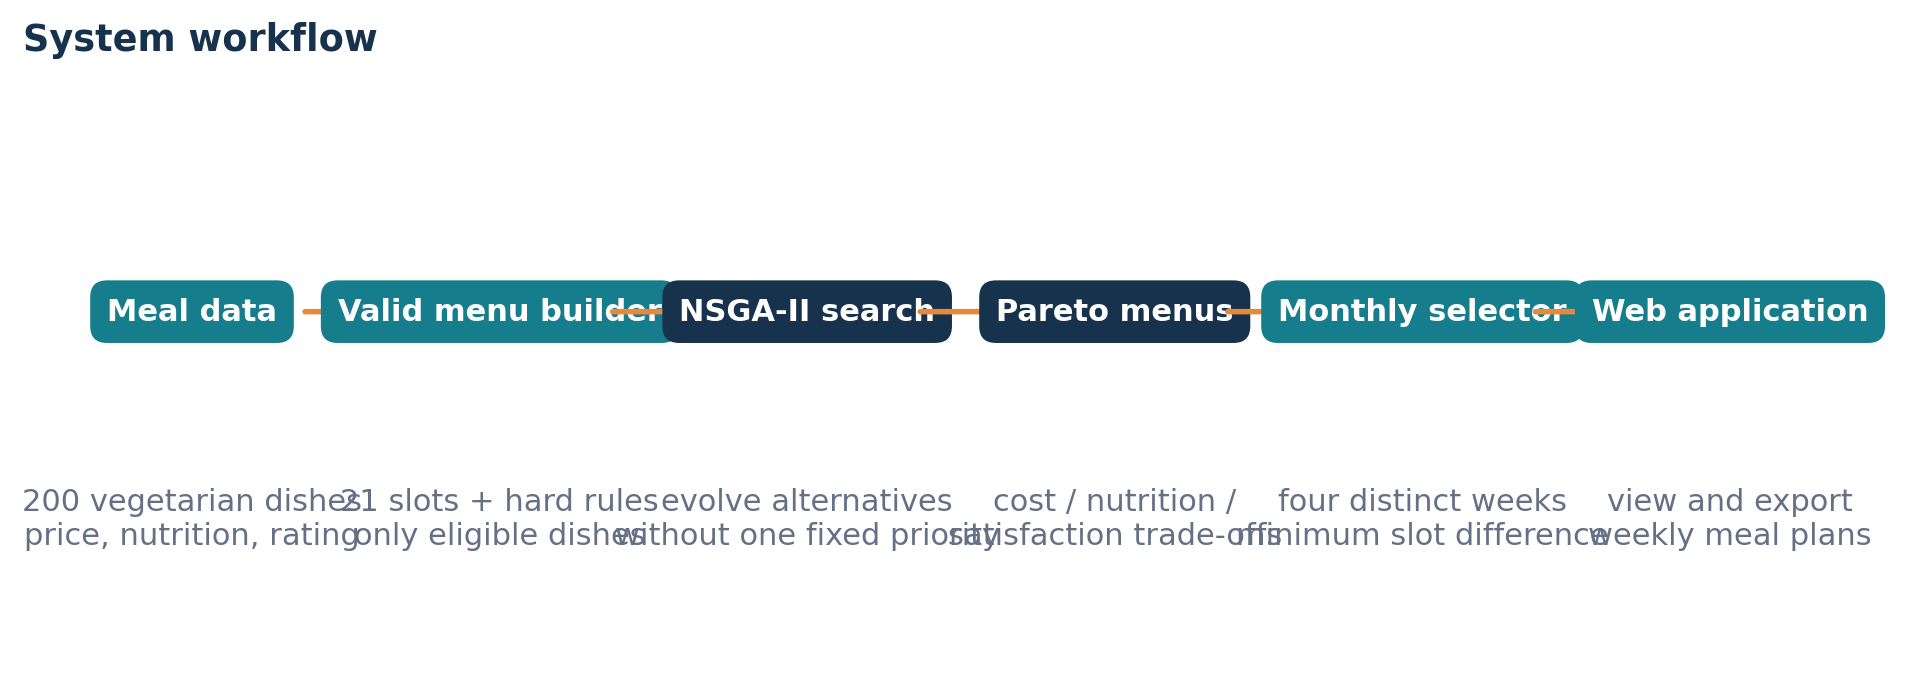
\includegraphics[width=\textwidth]{figures/system_workflow.png}
\caption{End-to-end workflow of the proposed system.}
\label{fig:workflow}
\end{figure}

\section{System workflow}
\begin{enumerate}
\item Load and validate the meal data.
\item Create an initial population using only meals eligible for each slot.
\item Evaluate cost, nutrition deviation, dissatisfaction and constraint violations.
\item Evolve candidates using NSGA-II until the configured generation limit.
\item Keep only feasible, non-dominated and unique weekly menus.
\item Select four weekly plans that differ by at least seven of the 21 slots.
\item Present the result through the API and web interface.
\end{enumerate}

\chapter{Soft Computing Technique}
\section{NSGA-II in simple terms}
NSGA-II is used because this project has several goals that pull in different directions. It works like a controlled ``survival of good alternatives'' process. A population of possible weekly menus is evaluated. Menus that are clearly worse on every objective are removed, while menus offering a meaningful trade-off are retained. Crossover exchanges choices between two menus, and mutation replaces a choice with another meal that fits the same slot.

The result is a Pareto set. A menu is non-dominated when no other feasible menu is at least as good in all objectives and better in one. This is valuable for a mess committee: it can choose, for example, a lower-cost plan or a plan closer to nutrition targets after seeing the trade-off.

\section{Objectives and constraints}
All three objectives are minimized. The expressions are intentionally compact because the main purpose is understandable planning.
\begin{align*}
f_1 &= \frac{\text{total weekly meal cost}}{7} \\[-2pt]
f_2 &= \frac{1}{7}\sum_{d=1}^{7}\left(\frac{|C_d-C_T|}{C_T}+\frac{|P_d-P_T|}{P_T}\right) \\[-2pt]
f_3 &= \text{average}(5-\text{rating}) + \text{configured repetition penalty}
\end{align*}
Here, $C_d$ and $P_d$ are a day's calories and protein; $C_T=2000$ kcal and $P_T=50$ g are provisional targets. Hard constraints are different from goals: a candidate is rejected if it has the wrong number of choices, an invalid slot, non-vegetarian meal, daily calories outside 1500--3000 kcal, daily cost above INR~80, or a repeat within the configured three-day window.

\section{Algorithm outline}
\begin{enumerate}
\item Build 21 slot-specific lists of eligible meal indices.
\item Randomly assemble initial menus from these lists.
\item Evaluate all objectives and constraint violations for every menu.
\item Rank feasible menus by non-domination and preserve diversity on the front.
\item Create new menus with same-slot crossover and slot-valid mutation.
\item Repeat evaluation and selection for the configured generations.
\item Return unique feasible non-dominated menus and diagnostics.
\end{enumerate}

\chapter{Dataset / Input Data}
\section{Data source and attributes}
The authoritative file is \texttt{data/hostel\_meal\_dataset\_cleaned.csv}. It contains 200 affordable vegetarian meal options from North Indian, South Indian, Gujarati, Maharashtrian and Indo-Chinese styles. Each row contains 20 fields, including meal ID, name, cuisine, eligible meal types, cost per serving, calories, protein, carbohydrate, fat, rating, preparation time, kitchen load and allergens.

\begin{table}[H]
\centering
\caption{Important inputs and outputs.}
\begin{tabularx}{\textwidth}{lY}
\toprule
\textbf{Item} & \textbf{Description}\\ \midrule
Input menu & 21 integer meal indices: 7 days $\times$ 3 meal slots\\
Input data & 200 vegetarian meal records with estimated nutrition and cost\\
Output & Feasible weekly menus, objective values, constraint report and stable 21-meal signature\\
Monthly output & Four selected weeks, pairwise slot differences, cost and frequency summary\\
\bottomrule
\end{tabularx}
\end{table}

\section{Preprocessing and limitations}
The dataset is sorted by \texttt{meal\_id} so that indices are reproducible. Meal-type eligibility is parsed to build slot-specific candidates. The current records are all vegetarian. Nutrition is recipe-estimated, and all rating counts are zero because ratings are synthetic. These choices are acceptable for a prototype but should be replaced by mess-specific recipes, serving sizes and genuine feedback before operational use.

\chapter{Implementation}
\section{Technology stack}
The optimizer is implemented in Python 3.10+ using pandas and NumPy for data handling, pymoo for NSGA-II, and matplotlib for saved experiment figures. FastAPI exposes the planning logic as HTTP endpoints. The student-facing interface uses React, TypeScript and Vite. Streamlit is retained as a research interface. Tests use pytest.

\section{Configuration}
\begin{table}[H]
\centering
\caption{Main prototype settings. These are configurable assumptions, not dietary prescriptions.}
\begin{tabular}{lll}
\toprule
\textbf{Setting} & \textbf{Value} & \textbf{Role}\\ \midrule
Weekly slots & 21 & 7 days $\times$ breakfast, lunch, dinner\\
Daily cost cap & INR~80 & hard limit\\
Calories & 1500--3000 kcal & hard daily range\\
Nutrition targets & 2000 kcal; 50 g protein & soft planning goals\\
Repetition window & 3 days & nearby repeats rejected\\
Monthly minimum difference & 7 slots & prevents similar weekly plans\\
Benchmark NSGA-II & population 40; 12 generations & ten-seed experiment\\
\bottomrule
\end{tabular}
\end{table}

\section{Implementation notes}
The chromosome uses integers rather than floating-point values because each gene means ``choose this meal row.'' Crossover swaps genes at the same slot, and mutation selects a replacement from the same slot's eligible list. This small design decision prevents an invalid breakfast/lunch/dinner conversion from being introduced by the optimizer. The evaluator remains the source of truth: the optimizer and baselines use the same constraint checks.

\chapter{Experimental Setup \& Analysis}
\section{Experiment design}
The checked-in ten-seed benchmark used the same dataset and hard rules for three approaches: NSGA-II, random feasible search, and greedy cost selection. NSGA-II used population size 40 and 12 generations. For each method, the recorded measures included runtime, feasible candidate count, non-dominated count, daily cost, calories, protein and deviation measures.

The comparison should be read carefully. NSGA-II evaluated roughly 480 candidates per run, whereas the random search and greedy baseline used different search budgets. Therefore, the experiment is evidence that the implementation behaves consistently under this setup; it is not proof that NSGA-II is always superior.

\begin{figure}[H]
\centering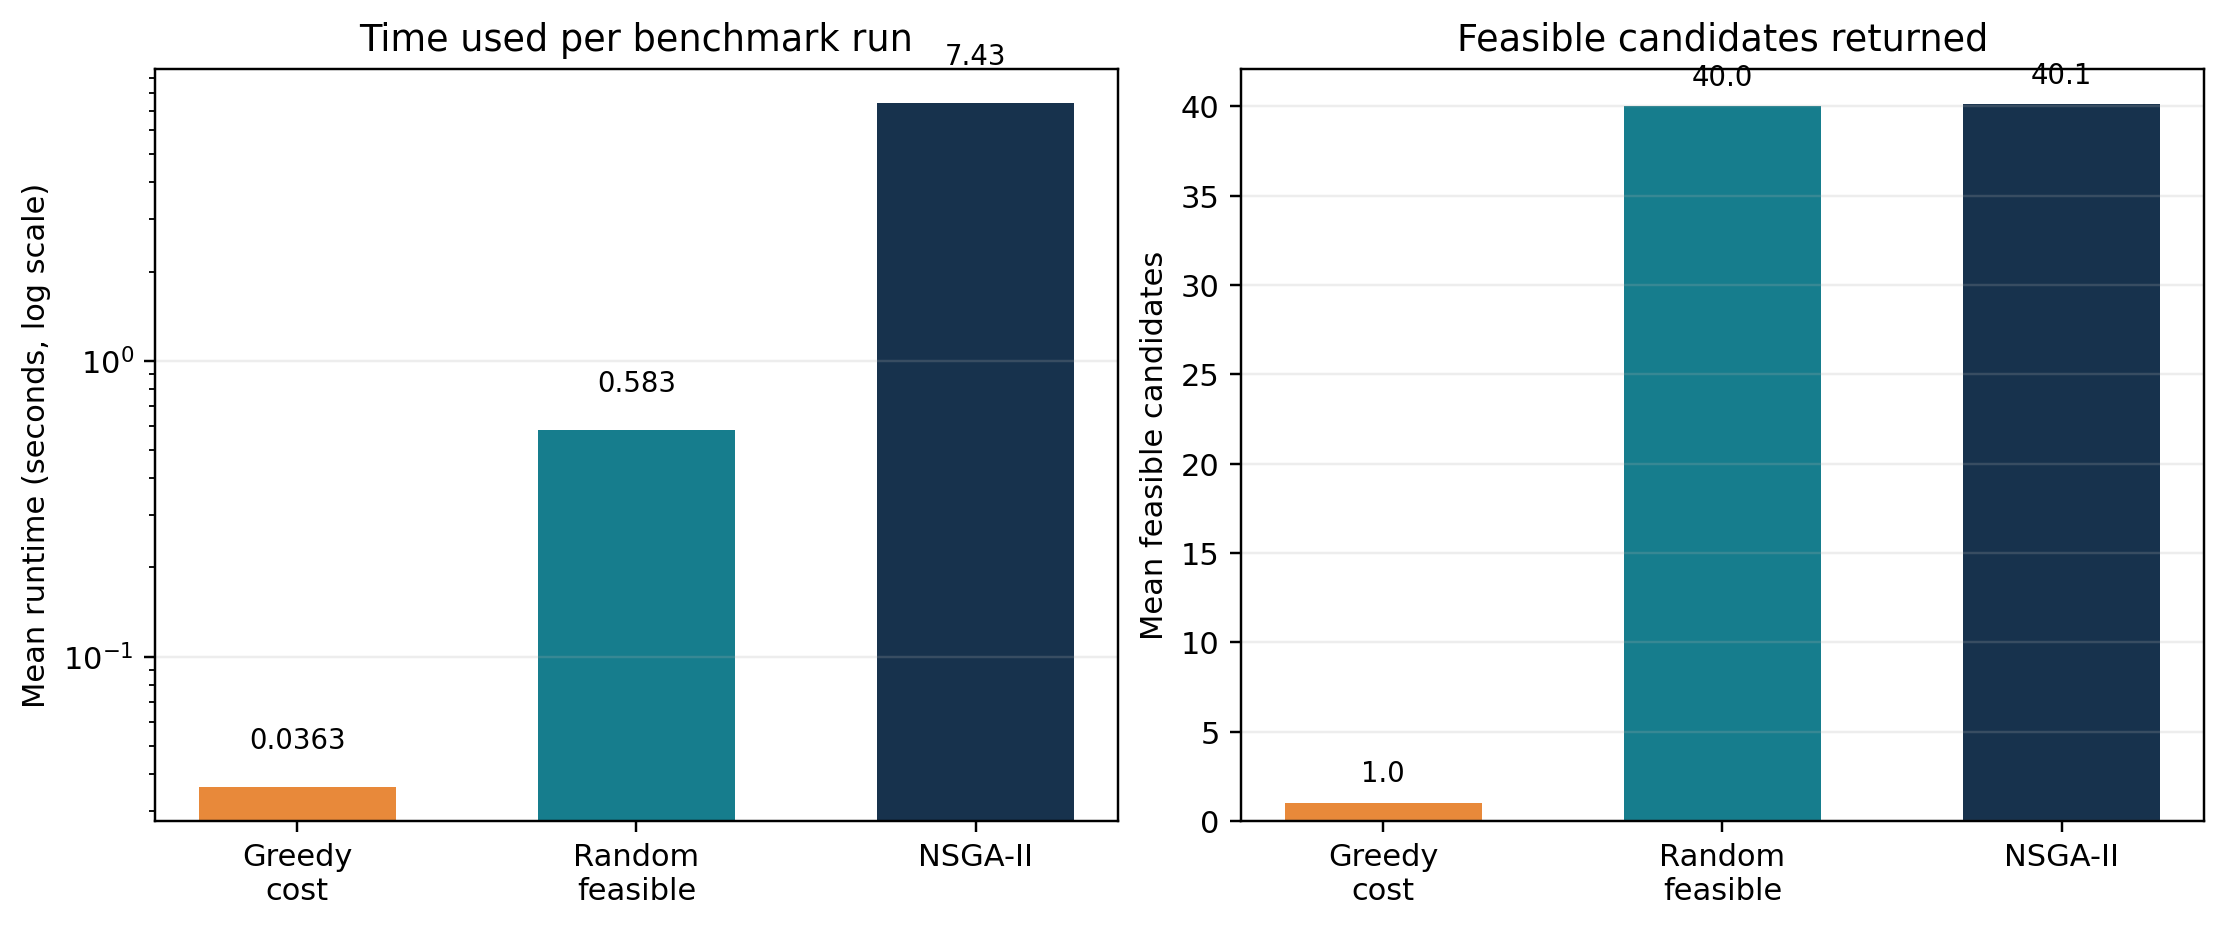
\includegraphics[width=0.94\textwidth]{figures/benchmark_comparison.png}
\caption{Measured ten-seed benchmark: runtime and feasible candidate count. Runtime uses a logarithmic scale.}
\label{fig:benchmark}
\end{figure}

\chapter{Results \& Discussion}
\section{Benchmark results}
\begin{table}[H]
\centering
\small
\caption{Mean values from the checked-in ten-seed benchmark.}
\begin{tabular}{lrrrr}
\toprule
\textbf{Method} & \textbf{Runtime (s)} & \textbf{Feasible} & \textbf{Cost/day} & \textbf{Non-dominated}\\ \midrule
Greedy cost & 0.036 & 1.0 & INR~75.71 & 1.0\\
Random feasible & 0.583 & 40.0 & INR~78.90 & 13.2\\
NSGA-II & 7.430 & 40.1 & INR~78.90 & 13.2\\
\bottomrule
\end{tabular}
\end{table}

The greedy method is fastest and has the lowest average cost, as expected because cost is its only priority. It produces one option, so it offers no meaningful choice. NSGA-II takes longer because it repeatedly evaluates and compares a population, but it produces a set of alternatives. In this particular run, NSGA-II and random feasible search have matching mean summary values; this result should be reported honestly. The value of NSGA-II here is its structured Pareto search and diagnostics, not an exaggerated claim of numerical dominance under unequal candidate budgets.

\section{Monthly planning result}
The monthly smoke run built a pool of 23 feasible weekly candidates from two short NSGA-II runs. It selected four schedules after considering 4,845 valid diverse combinations. The selected monthly plan had a total estimated cost of INR~2,196, an average daily cost of INR~78.43, 21 distinct meals and a maximum meal frequency of 9. Every selected pair differs by 17--21 slots, comfortably above the required 7-slot threshold.

\begin{figure}[H]
\centering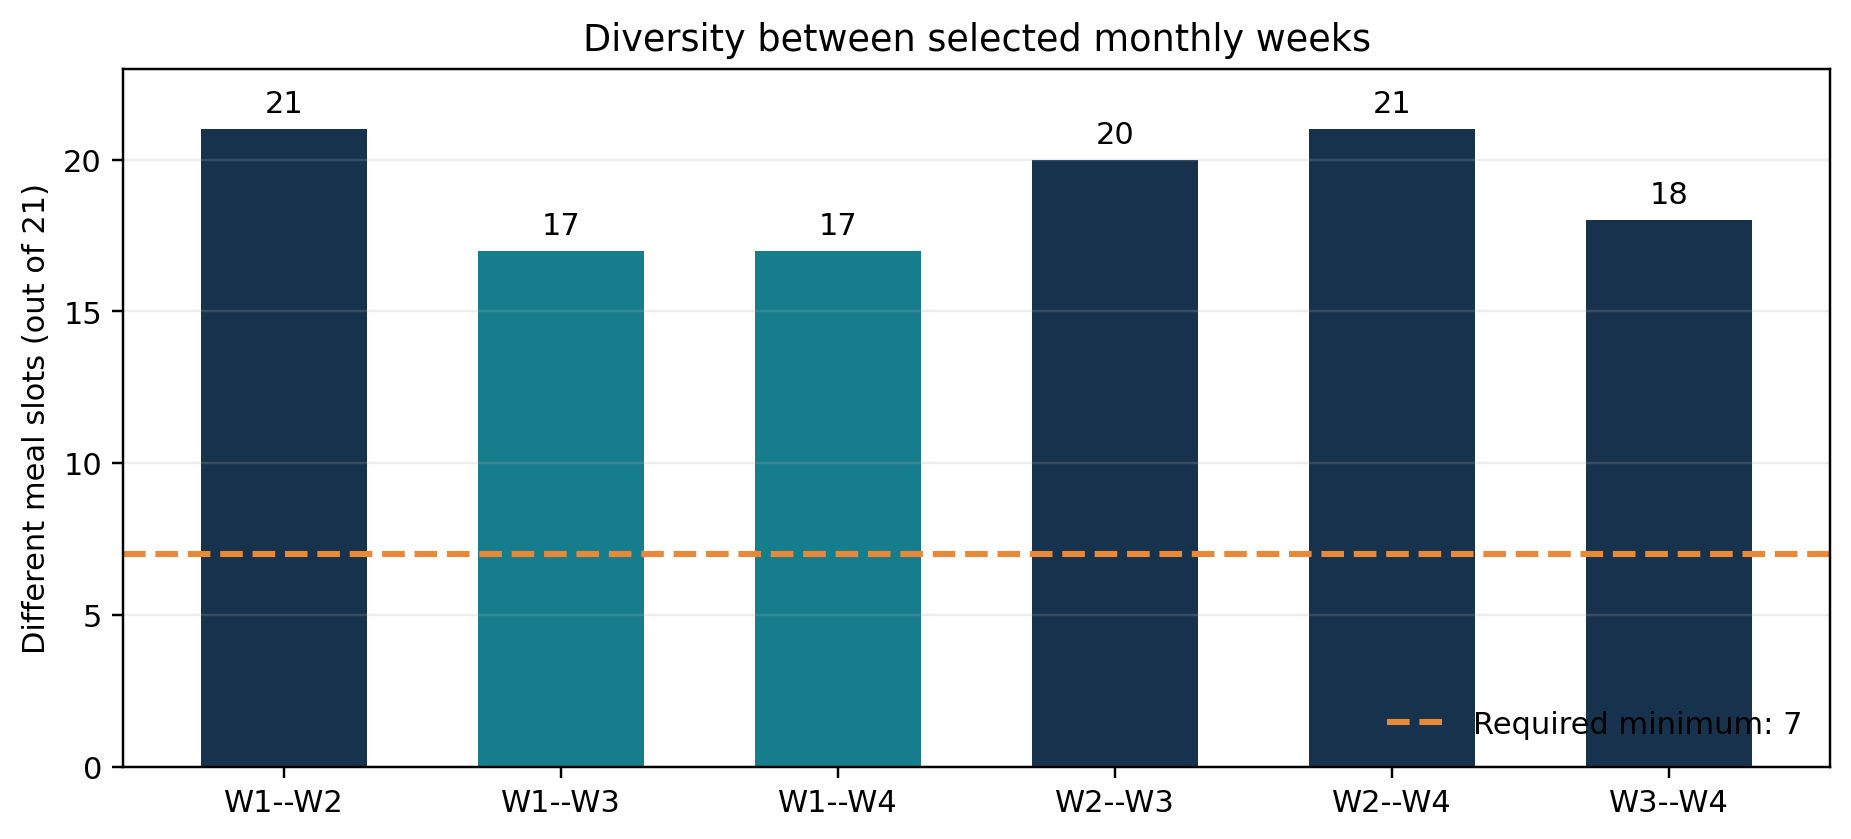
\includegraphics[width=0.88\textwidth]{figures/monthly_diversity.png}
\caption{Pairwise differences in the four-week selected plan.}
\label{fig:diversity}
\end{figure}

\section{Key observations}
\begin{itemize}
\item Feasibility was achieved in all ten benchmark runs for all three methods.
\item Multi-objective planning makes the trade-off visible; it does not replace a human decision about priorities.
\item The monthly layer effectively avoids near-duplicate weeks under the configured rule.
\item Average daily calories in these generated plans are close to the lower hard bound and below the 2000 kcal soft target. This is a useful signal to review the meal dataset and cost cap, not a reason to claim nutritional adequacy.
\end{itemize}

\chapter{Deployment}
\section{Deployment approach}
The project separates the presentation layer from the optimization logic. The React application calls a FastAPI adapter, which reuses the Python evaluator, optimizer, monthly scheduler and dataset. The same architecture can run locally for demonstration or be deployed with a static frontend host and a Python API service.

\begin{table}[H]
\centering
\caption{Deployment workflow.}
\begin{tabularx}{\textwidth}{lY}
\toprule
\textbf{Component} & \textbf{Responsibility}\\ \midrule
React + TypeScript frontend & Accepts planning inputs and displays generated schedules\\
FastAPI service & Receives requests and calls the existing optimization modules\\
Python optimizer & Loads data, checks rules, searches menus and returns results\\
Dataset / generated plans & Stores source meals and separates generated plans from benchmark artifacts\\
\bottomrule
\end{tabularx}
\end{table}

To use the system locally, the API is started with Uvicorn and the Vite frontend is started in a second terminal. The frontend sends a request to \texttt{/api}; the returned schedule can be viewed and exported. Before a public deployment, the provisional targets, serving-size data and feedback model must be reviewed with the actual mess administration.

\chapter{Conclusion}
This project delivers a working soft-computing approach to hostel menu planning. It represents a weekly menu as 21 choices, applies practical hard rules, and uses NSGA-II to return feasible trade-offs among cost, nutrition deviation and estimated dissatisfaction. It also adds a monthly selection layer so that four plans are not simply repeated copies.

The experiments confirm that the pipeline produces feasible results under the chosen settings and that the software records the information needed to inspect them. The main outcome is not a claim that the program can prescribe a perfect diet. It is a transparent planning assistant: it gives a mess manager several valid choices, shows why they differ, and keeps assumptions visible.

\chapter{Future Scope}
\begin{itemize}
\item Replace synthetic ratings with authenticated student feedback and confidence-aware preference scores.
\item Validate recipes, serving sizes and nutrition values with the hostel kitchen and a qualified nutrition professional.
\item Add ingredient availability, kitchen capacity, seasonal pricing and allergy-aware constraints.
\item Support student dietary profiles, including vegan, Jain and medical restrictions after proper review.
\item Run a fairer larger benchmark with matched evaluation budgets and statistical reporting.
\item Add administrator approval, audit history and production deployment monitoring.
\end{itemize}

\chapter{References}
\begin{thebibliography}{9}
\bibitem{deb2002} K. Deb, A. Pratap, S. Agarwal and T. Meyarivan, ``A Fast and Elitist Multiobjective Genetic Algorithm: NSGA-II,'' \textit{IEEE Transactions on Evolutionary Computation}, vol. 6, no. 2, pp. 182--197, 2002.
\bibitem{ferguson2004} E. L. Ferguson, N. S. Darmon, U. T. Fahmida, C. Fitriyanti, T. B. Harper and M. J. Gibney, ``Design of optimal food-based complementary feeding recommendations and identification of key problem nutrients using goal programming,'' \textit{Journal of Nutrition}, vol. 136, no. 9, pp. 2399--2404, 2006.
\bibitem{pymoo} J. Blank and K. Deb, ``pymoo: Multi-Objective Optimization in Python,'' \textit{IEEE Access}, vol. 8, pp. 89497--89509, 2020. \url{https://pymoo.org/}
\bibitem{fastapi} S. Ram\'irez, ``FastAPI Documentation.'' \url{https://fastapi.tiangolo.com/}
\bibitem{react} Meta Open Source, ``React Documentation.'' \url{https://react.dev/}
\bibitem{project} R. Raval and D. Sojitra, \textit{Hostel Mess Menu Optimizer: Project source code, dataset and benchmark artifacts}, 2026. Repository material: \texttt{data/hostel\_meal\_dataset\_cleaned.csv}, \texttt{results/benchmark\_run\_004\_summary.csv}, and \texttt{results/monthly\_smoke.json}.
\end{thebibliography}

\appendix
\chapter{Appendix: Reproducibility Notes}
The reported ten-seed benchmark is stored in \texttt{results/benchmark\_run\_004\_summary.csv}; raw records are available alongside it. The monthly demonstration is stored in \texttt{results/monthly\_smoke.json}. The usual development configuration is Python 3.10+, with packages listed in \texttt{pyproject.toml}. A fixed seed can be supplied to reproduce a run in the same pymoo environment. Because NSGA-II is stochastic, a different seed may produce another valid trade-off set.

\end{document}
